\chapter{Introduction} \label{ch:intro}
A guiding principle in the study of physics is that of limiting behavior.
When approaching any new problem or system, a great deal of insight may be achieved by first considering the most extreme examples.
For the field of ultracold atomic physics, this extreme has been the pursuit of near zero-energy atomic and molecular gases, which has proven to be an incredibly fruitful endeavor.
Specifically, the development of ultracold and quantum degenerate neutral gases has allowed us to consider the quantum nature of matter, and its interaction with external fields, in the few-body and many-body regimes \cite{gps08,Kohler2006,wbz99,ccg11,swm10,bdz08,Chin2010,Bertelson2007,mmn11,bdz08}.

Rapid advancement in the ability to laser cool and trap atoms \cite{mvs99,mvs99,psm02} has led to a number of notable achievements in recent years, including the creation of novel macroscopic states of quantum matter such as Bose-Einstein condensates (BEC) and degenerate Fermi gases \cite{aem95,Bradley1995,dma95,DeMarco1999,zhg03,MartinezdeEscolar2010,Mickelson2010ja,dym10,stg10}, the observation of the BEC-BCS crossover and quantum phase transitions \cite{rgj04,zss04,cba04Science,Bourdel2004,grj03,gme02,jsg08,Snoke2002,zbb14}, as well as the formation of macroscopic ensembles of ro-vibrational ground state molecules \cite{rtb03,Jones2006, Reinaudi2012,Stellmer2012,nom08,Lang2008}.

Each of these successes has been enabled by taking advantage of the precision control and manipulability that is accessible in ultracold atomic gases.
In particular, the use of external fields to dynamically influence the evolution and occupation of quantum states within an atomic gas has become an invaluable addition to the atomic physicist's toolbox \cite{Chin2010}.
An example of such a process is photoassociation, whereby one or more resonant or near-resonant light fields is used to couple internal states of a gas of interacting atoms.
By absorbing one or more photons from the light field(s), the initially free atoms may then associate and form bound molecular states, leading to occupation of a new quantum state \cite{Kohler2006, Jones2006, Burnett2002}.

	\begin{figure} 
		\centerline{
		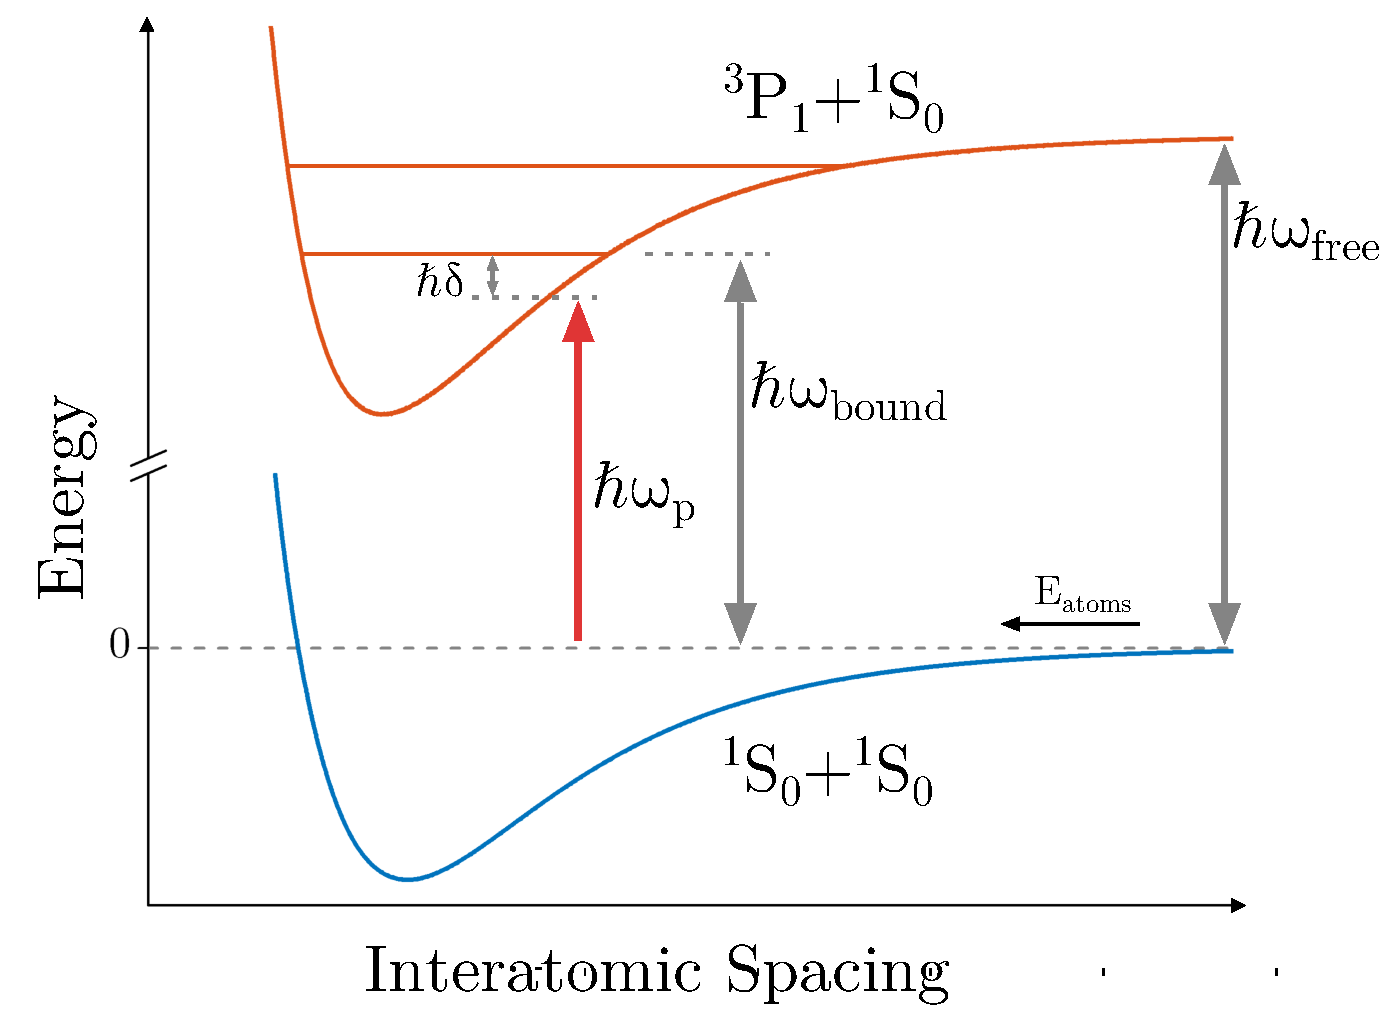
\includegraphics[width=0.6\textwidth]{PAschematic.pdf}}
		\caption{The photoassociation process}{Two atoms colliding with energy, E$_\text{atom}$, on a ground state potential in the presence of a photoassociation light field of frequency, $\omega_p$. This process will associate the two free atoms when the photoassociation light energy matches the energy difference between the incoming state and excited molecular state, $\hbar \omega_\text{p} = \hbar \omega_\text{free} - \hbar \omega_\text{bound}$.}
		\label{fig:1pasSch}
	\end{figure}
For neutral atoms, interactions between particles occur primarily at interparticle separations $<\!100\,\text{a}_0$, where $\text{a}_0$ is the Bohr radius \cite{Chin2010}.
These interactions give rise to the potential well that supports bound states, as shown in Fig.\,\ref{fig:1pasSch}.
This figure outlines a typical example of photoassociation using a single light field, known as one-photon photoassociation.
In this example, absorption of one photon will promote the internal energy of one atom of the colliding pair up to an excited potential.
Thus, when the laser frequency is appropriately tuned to a bound state energy, this absorption results in the creation of an excited weakly-bound molecular state.
The formation of this molecule is followed by spontaneous or stimulated decay, typically resulting in loss of both atoms from the trap.
Detection of atom loss is commonly observed as evidence of photoassociation and thus spectroscopy may be used to search for bound-state resonances.
The process of photoassociative spectroscopy (PAS) typically involves scanning the photoassociation (PA) laser frequency to the red of the free-atom asymptote.
This yields a series of molecular resonance energies progressively further from the free-atom excited state, which correspond to increasingly more deeply bound molecular states and consequently molecules with shorter bond lengths.
This reduction of the spatial extent of the deeply-bound molecular wavefunctions is important as it impacts the likelihood of association of the initial free-atom state to the final molecular state via overlap of the wavefunctions.
Thus, photoassociation of free atoms favors the creation of weakly-bound molecular states due to the long-range nature of the initial scattering wavefunctions which preferentially overlap with weakly-bound molecular states having large spatial extent.
Moreover, molecular states with small binding energies exhibit similar characteristics of the constituent free atoms, while more deeply bound molecules exhibit structure and properties reflective of the properties of the short-range atomic potential \cite{Jones2006}.

Using photoassociative spectroscopy in ultracold gases, the binding energy of molecular states may be directly measured.
These measuremenets reveal details about the short-range interaction potential between atoms and may be used to determine parameters such as the interparticle scattering length that characterizes the free-atom scattering behavior.

By adding an additional light field, two-photon photoassociation may be used to populate excited molecular states of the ground state potential.
This technique has proven to be an incredibly precise way to discern information about the collisional properties of ultracold atomic gases \cite{MartinezDeEscobar2008, Aman2018}.

However, the direct coupling of free atoms to the most deeply bound molecular states is not an efficient process and generally requires the use of additional photoassociative steps.
These may include STIRAP or preferential decay from excited-molecular states as has been recently demonstrated \cite{Reinaudi2012, cbc17, Stellmer2012, Ciamei2017}.
Ro-vibrational ground state molecules are interesting as their use has been proposed for precision measurements of variations of the proton-electron mass ratio \cite{zky08, Kotochigova2009} and the fine structure constant \cite{Beloy2011}. 


\section{Halo molecules} \label{sec:halo}
For some atomic species, external magnetic fields may be used to create weakly bound molecular states through the use of magnetic Feshbach resonances \cite{Kohler2006, Chin2010}.
These scattering resonances are the result of coupling between free scattering states (called open channels) and bound states (closed channels) where the scattering and bound states lie on two separate atomic interaction potentials with differential magnetic moments.
When the closed channel is swept through the threshold energy of the open channel, a weakly bound molecular state known as a Feshbach molecule is formed \cite{cbk03, grj03,hkm03,rtb03,sph03}.
Additionally, if these Feshbach molecules are created with the closed channel just below threshold they behave as exotic long-range molecules known as halo molecules \cite{Kohler2006}.
These molecules feature wavefunctions that extend far into the classically forbidden region.
Such states may be characterized by the large positive value of the free atom scattering length $a$ that is related to the binding energy of the halo molecule by
\begin{equation}
	E_b = -\frac{\hbar^2}{2 \mu a^2}
\end{equation}
where $\mu$ is the reduced mass of the atom pair.

	\begin{figure}
		\centerline{
		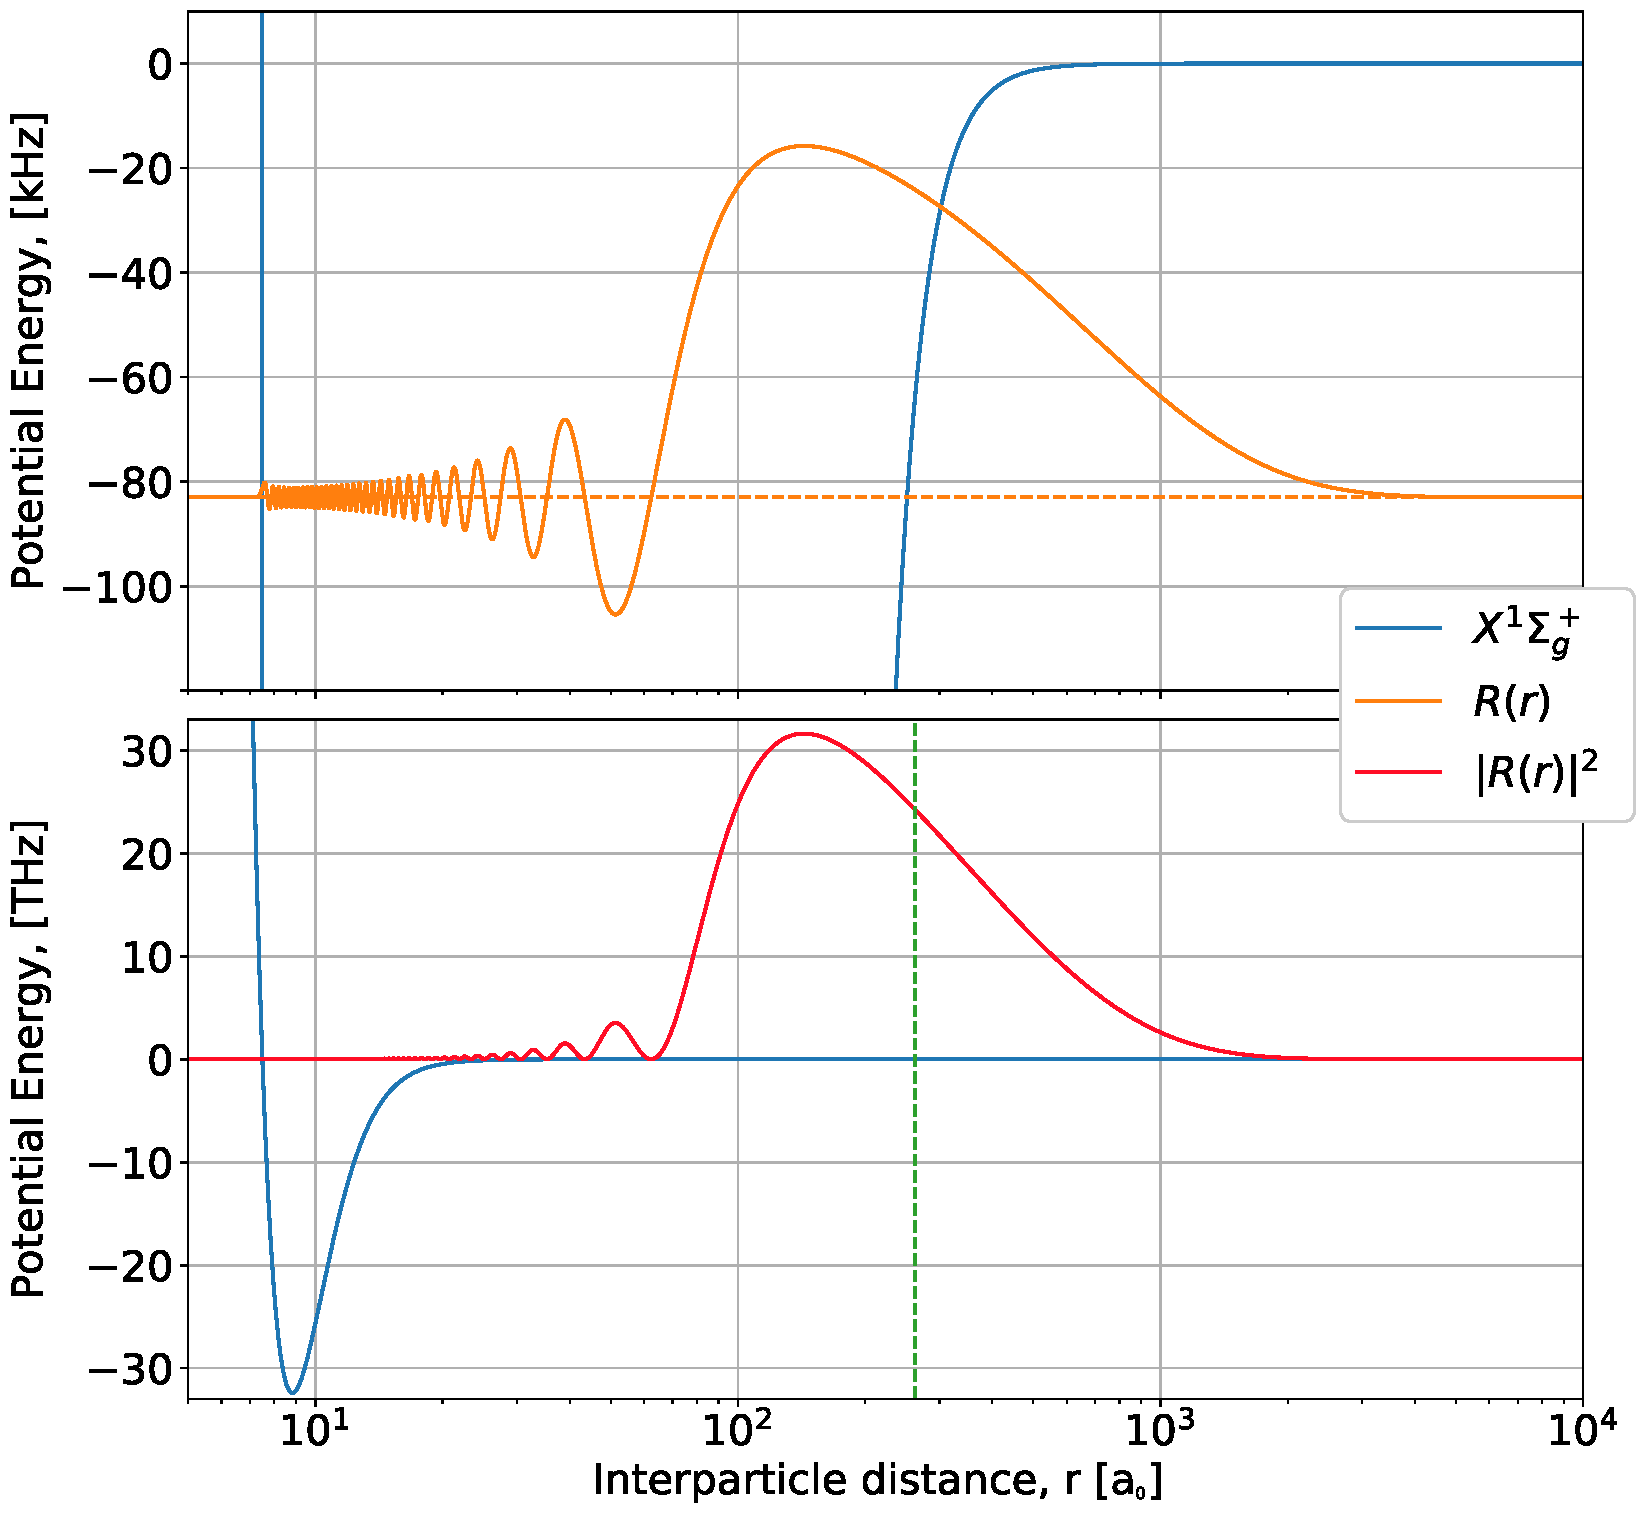
\includegraphics[width=\textwidth]{86halo.pdf}}
		\caption{$^{86}$Sr$_2$ halo radial wavefunction}{The extent of the strontium-86 halo radial wavefunction, $R(r)$, is shown compared to ground state potential. The complete bound state wavefunction is given by $\psi(\vec{r})=Y_{0,0}(\theta,\phi)\frac{R(r)}{r}$, where $Y_{l,m}(\theta,\phi)$ is the spherical harmonic. The radial Schr\"{o}dinger equation is solved for $R(r)$ using the Johnson renormalized Numerov method \cite{Gibson2016, Johnson1978} with the X$^1\Sigma_g^+$ potential from Ref.\,\cite{Stein2010}. The vertical dashed line is placed at the classical turning point $r_\text{classical} \approx 260$\,a$_0$. Note, the difference in energy scales between the top and bottom plots. The wavefunction normalization applied to each plot is arbitrary and only for illustrative purposes.}
		\label{fig:86halo}
	\end{figure} 
This concept of a spatially extended, few-particle, halo system is well-known and has been applied in various fields such as nuclear and molecular physics, with the most well known examples being the deuteron and $^4$He$_2$ molecules \cite{lmk93,sto94,Kohler2006}.
In atomic physics, halo molecules exist as the least-bound state in the extreme case of a scattering resonance, of which Feshbach resonances are a particular type.
Halo malecules are interesting quantum states due to their spatially extended wavefunctions which reach well past the classical turning point, $r_\text{classical} \cong \left( \frac{2 \mu a^2 C_6}{\hbar^2} \right)^{1/6}$.
Fig.\,\ref{fig:86halo} shows the radial component of the $^{86}$Sr$_2$ halo wavefunction with a farthest extent $>\!1000$\,a$_0$.
Such halo systems are notable for their universality, whereby molecular properties such as size and binding energy can be parameterized by a single quantity, the $s$-wave scattering length $a$, independent of other details of the atom-pair interaction \cite{Kohler2006,bha06}. 
Additionally, Efimov trimers may also exist in systems near a scattering resonance, influencing dimer and atomic scattering properties and introducing additional universal phenomena \cite{bha07,nen17}.

%Ultracold halo molecules are often associated with magnetic Feshbach resonances \cite{Chin2010}.
In this work, we probe the naturally occurring halo state which exists in the absence of tuning with a magnetic Feshbach resonance. 
This extremely weakly-bound molecular state depends strongly on the long-range portion of the strontium interaction potential between atoms that determines atom-atom scattering properties.
%measurement of the binding energy should provide a precise estimate of the long-range $C_6$ coefficient.

There are important differences between halo molecules associated with magnetic Feshbach resonances and the naturally occurring halo molecule in $^{86}$Sr. 
With magnetic Feshbach resonances, the relevant scattering and bound molecular states lie on different molecular potentials and the halo state results from mixing of different states.
Measuring the properties of these engineered states may then be challenging.
Several techniques have been demonstrated to measure molecular binding energies such as single-photon magnetic-dipole transitions and RF or microwave spectroscopy \cite{Chin2010,cju05,thw95b}. 
Typically, this is done by first forming molecules through magneto-association and then driving bound-free or bound-bound transitions converting the halo molecule into a different state and observing this loss.
Other methods of measuring the binding energy include spectroscopy with an oscillating magnetic field \cite{thw95b}, a modulated optically controlled Feshbach resonance \cite{chx15}, and Ramsey-type measurements of atom-molecule oscillation frequencies \cite{ckt03}. 
These are powerful techniques for manipulating quantum gases of alkali metals and other open-shell atoms in systems where magnetic Feshbach resonances are readily accessible.
Strontium, however, due to its closed-shell electronic structure, lacks magnetic Feshbach resonances in the electronic ground state.
%It is also possible to efficiently populate halo states with evaporative cooling \cite{jba03} near a magnetic Feshbach resonance. 


\section{Properties of strontium} \label{sec:sr}
Strontium is an alkaline-earth element with four naturally occurring isotopes, three bosonic and one fermionic.
The two valence electrons in its outer shell may align their spin anti-parallel or parallel, giving rise to a singlet and triplet series, respectively, of states.
Thus, two laser cooling phases are required to cool strontium to $\approx\!1\,\mu$K.
The first using the strong dipole-allowed $\,^1S_0\,\rightarrow\,^1P_1$ transition at $461$\,nm and the second using the narrow intercombination line $^1S_0\,\rightarrow\,^3P_1$ transition at $689$\,nm \cite{Katori1999,Ido2000,Mukaiyama2003a,Loftus2004,Ciuryo2004,Nagel2005a,Mickelson2005}.
These laser cooling transitions, as well as required repumping transitions, are shown in Fig.\,\ref{fig:energyLevels}.
	\begin{figure} 
		\centerline{
		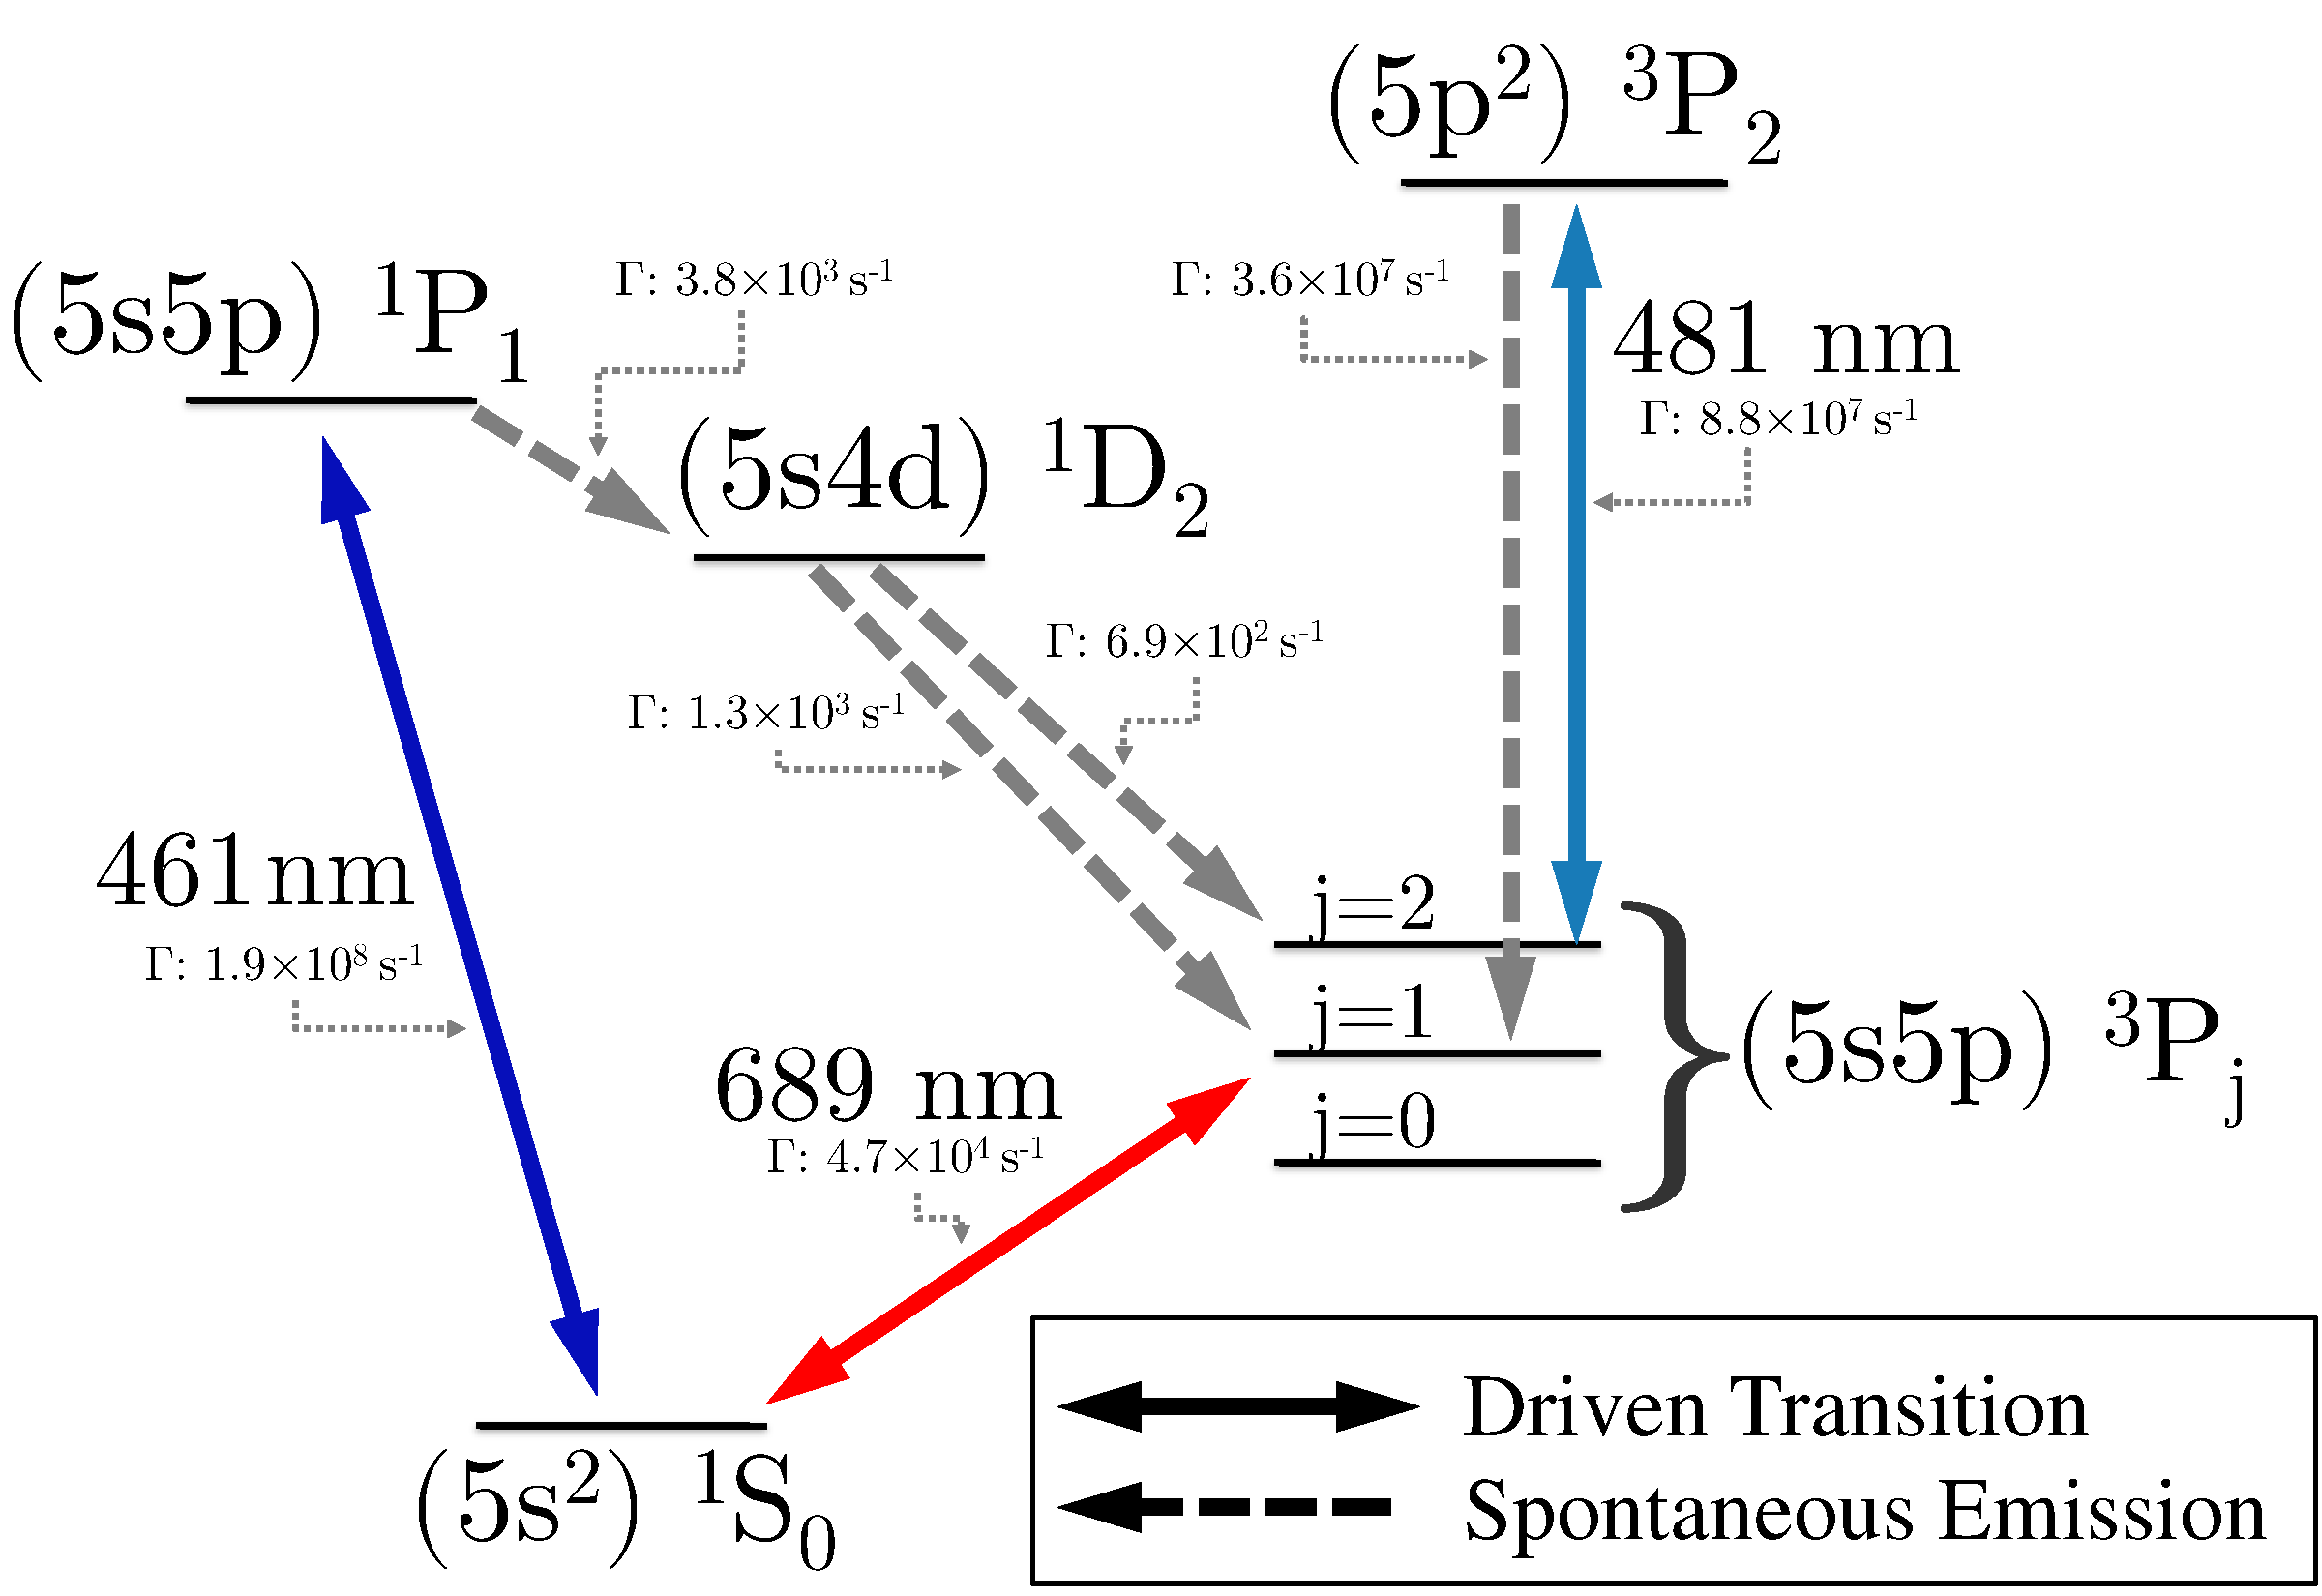
\includegraphics[width=\textwidth]{energy_level_diagram_v2.pdf}}
		\caption{Partial energy level diagram of strontium}{Shown are the relevant transitions and decay rates utilized to perform laser cooling and spectroscopy.}
		\label{fig:energyLevels}
	\end{figure}
	
The isotopic differences in strontium have important implications for their use in certain experiments.
In particular, the bosonic isotopes of strontium $^{88}$Sr, $^{86}$Sr, and $^{84}$Sr have no nuclear spin, $\vec{I}=0$.
This lack of hyperfine structure results in a single ground state potential, which greatly simplifies the treatment of collisions and scattering for these atoms.
Conversely, the fermionic isotope $^{87}$Sr has a large nuclear spin, $\vec{I}=9/2$, which when combined with the lack of electronic angular momentum in the ground state, results in a high degree of symmetry that must be considered when considering the behavior of these atoms during collisions.
This $SU(N)$ symmetry of $^{87}$Sr has led it to become a popular candidate for proposals exploring exotic phases of quantum magnetism \cite{Beverland2016,cre14,Chen2015}.

%From this measurement we derive estimates of the strontium scattering lengths (Table \ref{tab:sWaveComp}) \cite{Aman2018}.
In addition to the differences in quantum statistics and shifts of transition frequencies between isotopes, the homonuclear $s$-wave scattering lengths range from $-2\,$a$_0$ for $^{88}$Sr to $\sim\!800\,$a$_0$ for $^{86}$Sr.
Importantly for this work, we use the isotope with the largest homonuclear scattering length, strontium-86, to measure the binding energy of the least-bound state of the ground state potential via two-photon photoassociation performed near the narrow intercombination line $^1S_0\,\rightarrow\,^3P_1$ transition.
A considerable number of studies have previously reported photoassociation near this transition due to the availability of laser sources near $689\,$nm and the reduced off-resonant scattering rate that may be acheived when detuning from resonance.
The most abundant isotope, $^{88}$Sr, has been studied extensively in the context of narrow-line photoassociation, including one-photon PAS in a lattice \cite{Zelevinsky2006,McGuyer2013}, excitation of coherent Rabi oscillations between atomic and molecular condensates \cite{Yan2013b}, and the observation of optical Feshbach resonances \cite{Yan2013c, Blatt}.
Two-photon PAS experiments were also performed in $^{88}$Sr using this transition to measure the least-bound state of the X$^1\Sigma_g^+$ potential \cite{MartinezDeEscobar2008}.
Additionally, related techniques have produced more deeply bound vibrationally excited molecules in the electronic ground state using $^{88}$Sr \cite{Reinaudi2012, McGuyer2014, McGuyer2015a, rom12} and $^{84}$Sr \cite{Stellmer2012} trapped in optical lattices.
Finally, one-photon photoassociation spectroscopy has been used to probe the excited state molecular binding energies in bulk trapped gases near the intercombination transition in $^{86}$Sr \cite{Borkowski2014a, Reschovsky} and $^{84}$Sr \cite{Stellmer2012, Reschovsky}.

\section{Thesis Outline} \label{sec:outline}
This thesis will describe our work probing the weakly bound halo state of strontium-86.
Chapter 2 will outline our standard laser cooling and trapping procedures for producing samples of ultracold strontium at $\approx1\,\mu$K in an optical dipole trap. 
Additionally, the experimental apparatus and systems for trapping will be discussed.
Chapter 3 will develop the theoretical underpinnings of the photoassociation process that has a rate dependent on the spatial and thermal distribution of the atoms as well as the dynamical coupling provided by the applied PAS light fields.
Furthermore, this chapter explores atomic collisions and the importance of short-range interactions in determining the long-range behavior of scattering states.
In chapters 4 and 5, we present our findings from experiments probing the $^{86}$Sr$_2$ halo molecule.
The first experiments are performed in a high-intensity regime where we observed non-linear scaling of loss features and AC Stark shifts on the order of the binding energy of the halo molecule.
Following this, we performed a complimentary set of experiments, being careful to stay in a weakly perturbing regime, where we precisely determined the binding energy of the halo molecule accounting for several different possible shifts of the resonance energy.
This binding energy is then used to estimate improved scattering lengths for all isotopes of strontium.
Chapter 6 describes the installation and characterization of a $532$\,nm lattice laser system.
This system will be indispensable for our future work investigating quantum magnetism with fermionic strontium-87 as well as for studies of the properties of halo molecules and future work.
Further discussion of our proposed work will be given in chapter 7, along with concluding remarks.






%%%%%%%%%%%%%%%%%%%%%%%%%%%%%%%%%%%%%%%%%%%%%%%%%%%%%%%%%%%%%%%%%%%%%%%%%%%%%%%%%%%%%%%%%%%%%%%%%%%%%%%%%
%In  through short-range collisions.
%
%
%The laser light may then
%
%leading to coupling of the internal states of colliding atoms.
%This collisional interaction may then cause the atoms may .
%
%
%which leads to a change of the quantum state of particles
%
%This process connects internal states of colliding atoms using optical fields,
%
%whereby colliding free particle atomic states, illuminated by resonant laser light, 
%
%
%whereby resonant laser light is used to illuminate a gas of colliding atoms.
%Interaction between the internal atomic states and the light field 

%studies aimed to control atomic interactions building from the photoassociative techniques developed in this thesis.
%	
%This spatial discrimination along with the precise energy required to couple to a bound state result in a flexible tool mapping out the wavefunction of the scattering state to find its $s$-wave scattering length.
%
%
%Deeply bound molecular states are, in general, quite complicated and demonstrate a multitude of resonance frequencies between various internal, vibrational, and rotational energies.
%Photoassociation of free atoms 
%
%
%PA favors physicist molecules
%A significant part of the interest in ultracold AP has been the nature of the molecular states which are reafily produced and studied using this technique.
%The degree to which the atom molecule connection can be explicilty made in practice depdns aon the 
%high vibrational level are call long range molecules and prove one exmaple of a physicist molecules moleucles that can be related to the properties of the constituent atoms.
%
%In the most extreme case, molecules with binding energies of $10$
%
%
%modies atomic collisions
%
%yields information on atomic collisions
%field of photoassociation in ultracold gases, wherein studies of molecular structure have revealed the most accurate descriptions of atomic interactions and have become a fundamental probe of the ultracold toolbox \cite{Jones2006}.

%From this discussion, we 
%PA can come in many forms (in a lattice, in a bulk gas, via dissociating molecules) Experimentally we observe PA by looking for trap loss \hl{doublon paper}.
% 
% 
%rabi oscilations between atomic and molecular condensates (cite ours and the lattice experiment that followed)

%are the primary trapping mechanism for many alkali atom experiments and when combined with appropriately polarized and near resonant light a magneto-optical trap (MOT) is a robust tool applicable to nearly all cold atomic physics experiments.
%Furthermore, the use of dynamic B-fields allows researchers to tune atomic interactions at a microscopic level using

%Surprisingly, this phenomena may be described by simple two-level models and has become a mainstay in many atomic physics laboratories.
%
%While magnetic tuning may lend itself to simple theoretical descriptions, the temporal and spatial control of optical fields is unmatched.